\documentclass{memoir}
\usepackage{lmodern}
\usepackage[utf8]{inputenc}
\usepackage[italian]{babel}
\usepackage{amsmath}
\usepackage{graphicx}

\graphicspath{{./draws/}}

%\title{How to write a Report\\ for the Project of Distributed Systems}
\title{Progetto di Sistemi Distribuiti}

\author{Dott. Diego Borsoi\\Dott. Filippo Callegari\\ DMIF, University of Udine, Italy}

\date{Version 0.1, \today}

\begin{document}


%\begin{titlingpage}
\maketitle
\begin{abstract}
The aim of this document is to describe how to write a report for the project-exam for the course Distributed Systems, at the University of Udine.
It is also a guideline for the development of the project itself.

This document is very brief and succint, and it is by no means comprehensive of all the informations that should be given about a software project. You are invited to supplement these guidelines as needed to best describe your work.
\end{abstract}
%\end{titlingpage}

\chapter{Introduzione}\label{ch:intro}

Il progetto in questione riguarda la creazione di un sistema distribuito per la comunicazione fra dispositivi all'interno di una rete sparsa, tramite l'utilizzo di eventi.

\section{Descrizione del problema}

Ogni dispositivo corrisponde ad un nodo della rete ed è caratterizzato da:
\begin{itemize}
\item \textbf{Id} : numero univoco del nodo.
\item \textbf{Stato} : tupla di variabili che rappresentano delle specifiche caratteristiche del nodo (es. temperatura di un sensore, stato di accensione di una termocoppia, ecc).
\item \textbf{Regole} : insieme di regole del tipo ECA (Event Condition Action) che possono attivarsi a seguito di un evento inviato al nodo. Queste regole possono essere di due tipi: locali, l'azione modifica solamente lo stato del nodo in cui si attiva, oppure globale, l'azione viene inviata a tutti i nodi della rete perché venga letta ed, in caso la valutazione della guardia associata sia positiva, eseguita.
\center$\{event;~condition;~action~|~\text{if}~guard~\text{then}~action\}$
\end{itemize}

Lo stato della rete si evolverà ogni qual volta un evento verrà attivato, andando a sua volta ad innescare eventuali nuovi eventi e creando quindi una sequenza di azioni a cascata.

\section{Struttura dell'implementazione}

La rete in questione ha una struttura a mesh sparsa (cioè ogni nodo sarà al più connesso a un numero di nodi molto basso, rispetto alla totalità).
I nodi sono idempotenti in modo tale da avere un sistema fortemente decentralizzato.
Le varie comunicazioni fra i nodi sono eseguite al di sopra di connessioni TCP, in tal modo possiamo garantire la consegna di ogni messaggio nell'ordine prestabilito.
Per quanto concerne invece le comunicazioni riguardanti il sistema di $heartbeat$ (TODO: link al capitolo), queste vengono eseguite utilizzando connessioni UDP.

\section{Trasparenze}\label{Trasparenze}

Di seguito sono descritte le trasparenze che concergono e sono implementate dal sistema:

\begin{description} 
\item[Trasparenza ai fallimenti:] nel momento in cui un nodo fallisce/si disconnette, il resto della rete continua a funzionare normalmente.
\item[Trasparenza alla scalabilità:] la rete può espandersi in dimensione senza che il funzionamento dei nodi vari.
\item[Trasparenza alla mobilità:] un nodo può spostarsi all'interno della rete senza che il funzionameto suo e degli altri nodi vada a modificarsi.
\end{description}

\section{Algoritmi}

Il sistema implementa solamente due algoritmi:
\begin{itemize}
\item \textbf{Flooding Algorithm:} viene usato per la comunicazione di un'azione a tutta la rete nel momento in cui in un nodo una regola globale viene attivata.
\item \textbf{Lamport clock (modificato):} viene utilizzata una versione modificata del Lamport clock per identificare i vari $flood$ eseguiti; questo clock viene incrementato solamente dall'invio (o ricezione) di un messasggio, e non dalle azioni interne ad un nodo.
\end{itemize}

Il sistema non implementa particolari algoritmi essendo che si vuole realizzare una rete distribuita dove ogni nodo conosce esclusivamente i vicini ed evolve il suo stato solamente a causa di eventi ricevuti tramite dei messaggi.

\section{Testing}

Per testare il sistema verrà utilizzata un'entità $Ambiente$, la quale simulerà: 
\begin{itemize}
\item la creazione iniziale della rete, caricando da dei file appositi la struttura degli stati, la lista di regole e la conformazione della rete
\item la scoperta di nuove connessioni
\item variazioni di variabili legate all'ambiente (es. temperatura registrata da un sensore)
\item fallimenti di nodi
\item ritardi nell'invio di messaggi fra nodi
\end{itemize}

Ogni modulo verrà testato singolarmente ed infine verranno eseguiti dei test completi del sistema.

\section{Piano di sviluppo}

Le future fasi di sviluppo seguiranno il seguente ordine:
\begin{enumerate}
\item Riunione con il committente per convalidare la risoluzione del problema
\item Implementazione ambiente virtuale per la gestione dei nodi 
\item Implementazione della struttura del nodo
\item Implementazione sistema $heartbeat$
\item Implementazione del sistema algoritmico
\item Test totale
\item Validazione
\end{enumerate}


%\section{Istruzioni}
%In this chapter you describe the main problem, and an idea of the solution.
%It is not necessary to be very detailed or formal, but it is important to explain which are the main aims and issues from the point of view of Distributed Systems:
%\begin{itemize}
%\item A description of the application.
%\item The overall structure of the implementation: how resources are deployed, which are the players, the r\^oles.
%\item The distributed system features (and the transparencies) and algorithms you intend to implement.
%\item Your plan for testing the system.
%\item A schedule for how you plan to carry out your design and implementation
%\end{itemize}

\chapter{Analisi}\label{ch:analisi}

In questo capitolo vengono descritti nel dettaglio requisiti funzionali e non funzionali della soluzione proposta.

\section{Requisiti Funzionali}

I requisiti funzionali individuati sono:
\begin{itemize}
\item \textbf{Categorizzazione di un nodo:} ogni nodo ha un tipo il quale ne identifica lo stato e le sue regole;
\item \textbf{Modifica delle regole di un nodo:} ogni tipo di nodo può avere le sue regole, codificabili attraverso la programmazione dello stesso;
\item \textbf{Modifica dello stato di un nodo:} ogni evento permette di avere o degli \textit{effetti locali} o degli \textit{effetti globali}:
	\begin{itemize}
	\item \textit{\textbf{effetti locali}}: la regola va a modificare lo stato interno;
	\item \textit{\textbf{effetti globali}}: la regola può modificare lo stato delle variabili interne, e può generare un evento sugli altri nodi;
	\end{itemize}
\item \textbf{Aggiunta dinamica di un nodo:} un nodo può essere aggiunto alla rete in qualsiasi momento senza perturbarne la dinamicità, limitando l'aggiornamento ai vicini a cui si collega.
\item \textbf{Esecuzione di un'azione ricevuta dai vicini:} nel momento in cui un nodo riceve un messaggio dai propri vicini esso va a verificare la soddisfacibilità della guardia (se presente) e nel caso di una valutazione positiva viene eseguita l'azione associata, andando quindi a modificare il proprio stato.
\item \textbf{Attivazione di una regola:} ogni qual volta avviene un cambiamento nello stato di un nodo, viene eseguito un controllo delle regole, per vedere se gli eventi generati possano attivare una o più regole del nodo; nel caso in cui una regola venga attivata, in base al tipo (locale o globale) viene portata a termine l'azione corrispondente.
\end{itemize}

\section{Requisiti Non Funzionali}

I requisiti non funzionali individuati sono:
\begin{itemize}
\item \textbf{Decentralizzazione:} nessun nodo ha il controllo dell'ordine degli eventi, grazie al fatto che ogni nodo è idempotente;
\item \textbf{Tolleranza ai guasti:} poichè tutti i nodi sono idempotenti, nel momento in cui un nodo si scollega dalla rete, la rete rimanente continua ad operare normalmente;
\item \textbf{Etereogenità:} fintanto che i nodi aggiunti utilizzano il protocollo descritto, qualunque nodo di qualunque tipo (hardware o categoria) potrà essere aggiunto alla rete;
\item \textbf{Scalabilità:} l'aggiunta dinamica dei nodi alla rete permette di scalare orizzontalmente con estrema facilità;
\item \textbf{Trasparenze:} le trasparenze implementate sono quelle descritte al capitolo precedente (paragrafo \ref{Trasparenze}).
\end{itemize}

%\chapter{Analysis}\label{ch:analysis}
%
%In this chapter, we describe in detail functional and non-functional requirements of a solution for the problem.
%
%\section{Functional requirements}
%Which functions must be offered to users / other programs?  Which are the input data and the output data? Which is the expected effect? 
%
%\section{Non functional requirements}
%Everything about mode and transparencies: availability, mobility, security, fault tolerance, etc.
%
%Are there execution time bounds? Minimum data rates?
%
%If requested, specific platforms/languages/middlewares requirements for the implementation can be decided here. (E.g.: if the project is on a SOA, we may request that functions are offered via SOAP or RESTful services). 



\chapter{Progetto}\label{ch:progetto}

In questo capitolo vengono descritti in modo più approfondito l'achitettura del progetto, i moduli, i protoclli e gli algoritmi utilizzati.

\section{Architettura logica}

Essendo tutti i nodi costruiti al medesimo modo, di seguito presentiamo la struttura di uno singolo di essi. 

\begin{figure}[h]
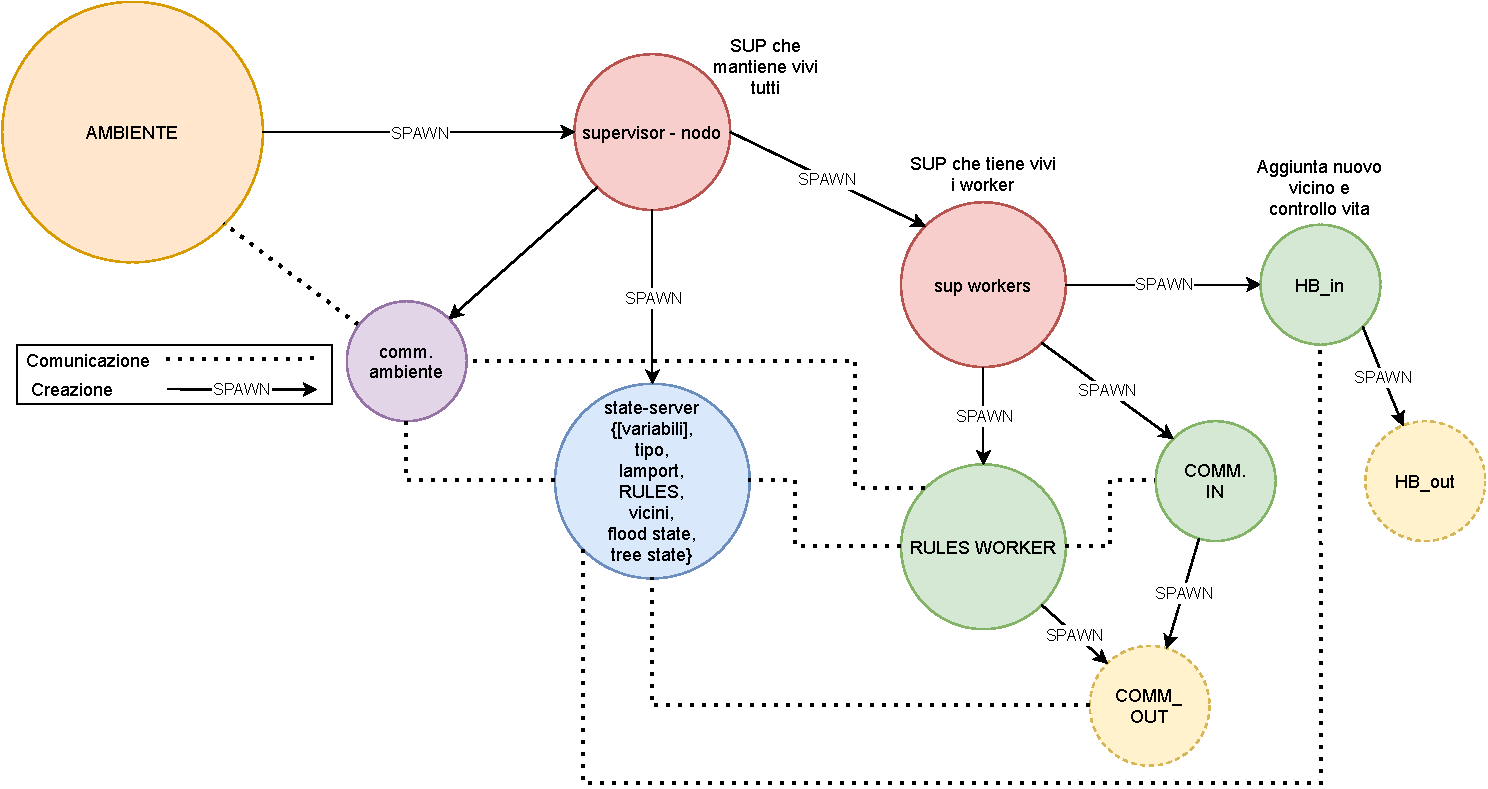
\includegraphics[scale=0.6]{draw_nodeworker.pdf}
\centering
\caption{Struttura gerarchica dei moduli di un nodo e visualizzazione delle connessioni fra di essi.}
\label{img:struttura_nodo}
\end{figure}


Come si può vedere dalla figura \ref{img:struttura_nodo}, ogni nodo è formato dai seguenti moduli:
\begin{itemize}
\item \textbf{Supervisor nodo:}
\item \textbf{State server:}
\end{itemize}

% TODO: cambiare environment in ambiente nel disegno
Come è stato accennato in precedenza verrà sviluppato un ulteriore modulo chiamato \textbf{\textit{Ambiente}}: questo modulo ...


\section{Protocolli ed algoritmi}
\section{Architettura fisica e deployment}
\section{Piano di sviluppo}


%This chapter is devoted to the description of the general architectures, and specific algorithms.
%
%\section{Logical architecture}
%Describe the components of your systems: modules/objects/components/services.
%For each component, describe the functionalities it implements, and by who is used.
%
%\section{Protocols and algorithms}
%Communication between components.  UML sequence diagrams go here.
%
%Also, put here a detailed description of distributed algorithms used to solve specific problems of the project.
%
%\section{Physical architecture and deployment}
%Which nodes and platforms involved, and where each component is deployed.
%
%\section{Development plan}
%Since it is difficult to predict just how hard implementing a new system will be, you should formulate as a set of ``tiers,'' where the basic tier is something you’re sure you can complete, and the additional tiers add more features, at both the application and the system level.

\chapter{Implementation}

Details about the implementation: every choice about platforms, languages, software/hardware, middlewares, which has not been decided in the requirements.


Important choices about implementation should be described here; e.g., peculiar data structures.


\chapter{Validation}

Check if requirements from Chapter~\ref{ch:analysis} have been fulfilled.
Quantitative tests (simulations) and screenshots of the interfaces are put here.


\chapter{Conclusions}

What has been done with respect to what has been promised in Chapters~\ref{ch:intro} and \ref{ch:analysis}, and what is left out.

\appendix

\chapter{Appendix}

In the Appendix you can put code snippets, snapshots, installation instructions, etc.


\chapter*{Evaluation}
Your system will be judged mainly on how it operates as a distributed system. The primary evaluation will be according to whether your system has the following attributes:
\begin{itemize}
\item  It should be an interesting distributed system, making use of some of the algorithms we have covered in class for distributed synchronization, replication, fault tolerance and recovery, security, etc.
\item The software should be well designed and well implemented, in terms of the overall architecture and the detailed realization.
\item You should devise and apply systematic testing procedures, at both the unit and systems levels.
\item The system should operate reliably and with good performance, even in the face of failures.
\end{itemize}
Important, but secondary considerations include:
\begin{itemize}
\item Time taken to do the project (the sooner the better, but do not miss details in order to end sooner)
\item  How nice is the application's appearance: does it have a nice interface or a compelling visual display?
\end{itemize}

\end{document}